\documentclass[tikz,border=10pt]{standalone}

\begin{document}
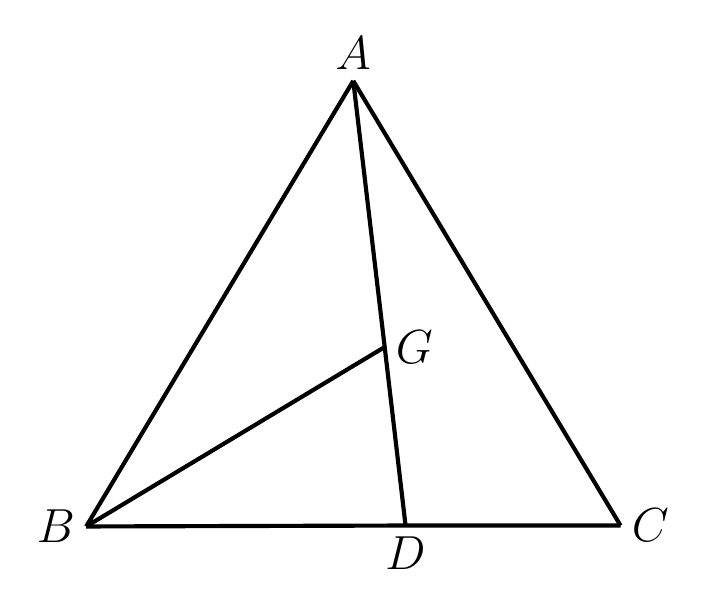
\begin{tikzpicture}[line width=1.5pt, line join=round]
\coordinate (A) at (0.000,2.827);
\coordinate (B) at (-3.392,-2.832);
\coordinate (C) at (3.394,-2.820);
\coordinate (D) at (0.664,-2.820);
\coordinate (G) at (0.399,-0.553);



  
  \draw (A) -- (B);
  \draw (A) -- (C);
  \draw (B) -- (D) -- (C);

  
  \draw (A) -- (G) -- (D);
  \draw (B) -- (G);

  
  \node[above] at (A) {\fontsize{16}{19.2}\selectfont $A$};
  \node[left] at (B) {\fontsize{16}{19.2}\selectfont $B$};
  \node[right] at (C) {\fontsize{16}{19.2}\selectfont $C$};
  \node[below] at (D) {\fontsize{16}{19.2}\selectfont $D$};
  \node[right] at (G) {\fontsize{16}{19.2}\selectfont $G$};
\end{tikzpicture}
\end{document}